\chapter{اللون والامتصاصية}\label{ch:g11:absorbance}

قارورة مشروب رياضي تتوهج بزرقة ساطعة على مقعد في قاعة رياضية. ولونها آتٍ من
صبغة ذائبة فيها، بضعة مليغرامات في لتر كامل: أقل بكثير من أن يوزن، وأقل بكثير
من أن يُرى جسمًا صلبًا. ومع ذلك على مختبر الأغذية أن يتحقق من هذا المقدار، لأن
الصبغة لا تُضاف إلا في حدود معيّنة. واللون نفسه هو المفتاح. فكلما زادت الصبغة
في \omterm{def:g2:mixing-and-dissolving:dissolve}{المحلول} زاد الضوء الذي يمتصه؛ والجهاز الذي يقيس مقدار ما يمتصه \omterm{def:g2:mixing-and-dissolving:dissolve}{المحلول} من
الضوء يقيس في الحقيقة تركيزًا.

\begin{recall}
\omterm{def:g10:concentration-and-dilution:mass-concentration}{التركيز الكتلي} \omterm{def:g10:concentration-and-dilution:molar-concentration}{والتركيز المولي} \omterm{def:g2:mixing-and-dissolving:dissolve}{لمحلول}؛ \omterm{def:g10:concentration-and-dilution:dilution}{وتخفيف} \omterm{def:g10:concentration-and-dilution:dilution}{محلول أم}؛ \omterm{def:g10:concentration-and-dilution:standard}{والسلّم المرجعي} من
المحاليل المعيارية الذي يُقارن به \omterm{def:g2:mixing-and-dissolving:dissolve}{محلول} مجهول
(\cref{ch:g10:concentration-and-dilution}).
\end{recall}

\begin{omfigure}
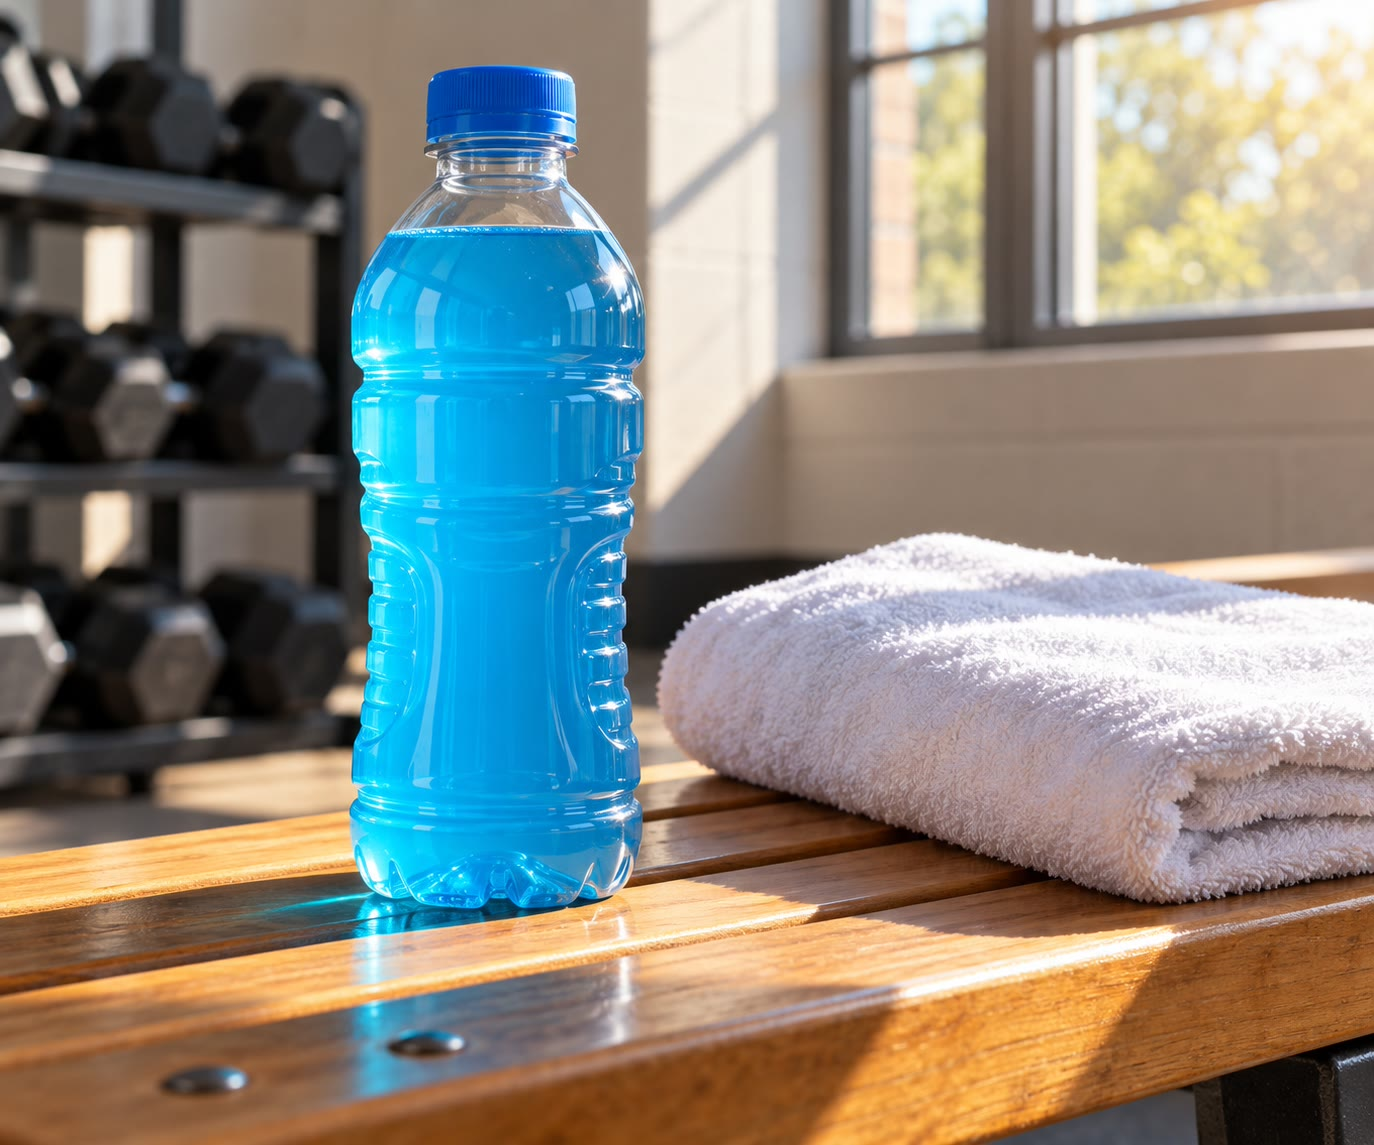
\includegraphics[width=0.5\linewidth]{images/book1/ai/g11-sports-drink.jpg}

{\small مشروب أزرق: لونه آتٍ من بضعة مليغرامات من الصبغة في
اللتر.}
\end{omfigure}

\section{لون المحلول}

الضوء الأبيض، مثل ضوء النهار، \omterm{def:g6:pure-substances-and-mixtures:mixture}{خليط} من كل ألوان قوس قزح. ويوافق كل لون طولَ
موجة، من نحو \qty{400}{nm} للبنفسجي إلى نحو \qty{750}{nm} للأحمر؛ ويشرح كتاب
الفيزياء ما طول الموجة، وهو هنا ليس إلا علامة على اللون. \omterm{def:g2:mixing-and-dissolving:dissolve}{والمحلول} الملون يمتص
جزءًا من الضوء الذي يعبره، وبعض الألوان أكثر بكثير من بعض؛ والعين ترى الألوان
التي تمر.

\begin{definition}[الألوان المتتامة]\label{def:g11:absorbance:complementary}
يكون اللونان \emph{لونين متتامين}\index{ألوان متتامة} إذا أعطى مزجهما ضوءًا
أبيض. وعلى دائرة الألوان يتقابل اللونان
المتتامان.
\end{definition}

\begin{omfigure}
\begin{tikzpicture}[font=\small]
  \foreach \a/\c/\n/\w/\t in {90/red!85!black/{أحمر}/{620--750}/white,
      30/orange/{برتقالي}/{590--620}/black, -30/yellow!90!orange/{أصفر}/{570--590}/black,
      -90/green!70!black/{أخضر}/{500--570}/white, -150/cyan!50!blue/{أزرق}/{450--500}/white,
      150/violet!80!blue/{بنفسجي}/{400--450}/white} {
    \fill[\c] (0,0) -- (\a-30:1.8) arc[start angle=\a-30, end angle=\a+30,
      radius=1.8] -- cycle;
    \node[text=\t, font=\small\bfseries] at (\a:1.2) {\n};
    \node[font=\footnotesize, align=center] at (\a:2.45) {\w\\ nm};
  }
  \fill[white] (0,0) circle (0.45);
  \draw[<->, thick, black!70] (90:0.5) -- (-90:0.5);
  \draw[<->, thick, black!70] (30:0.5) -- (-150:0.5);
  \draw[<->, thick, black!70] (-30:0.5) -- (150:0.5);
\end{tikzpicture}

{\small دائرة ألوان، مع أطوال موجات تقريبية. يتقابل اللونان المتتامان: الأحمر
والأخضر، والبرتقالي والأزرق، والأصفر
والبنفسجي.}
\end{omfigure}

\begin{proposition}[اللون المرئي]\label{prop:g11:absorbance:colour-seen}
\omterm{def:g2:mixing-and-dissolving:dissolve}{المحلول} الذي يمتص أساسًا لونًا واحدًا من الضوء الأبيض يبدو باللون المتمم
له.
\end{proposition}

\begin{proof}
نقبله: فالضوء الذي يمر هو الضوء الأبيض ناقصًا اللون الممتص، والعين ترى هذا
الباقي على أنه اللون المتمم.
\end{proof}

\begin{example}[صبغتان غذائيتان]\label{ex:g11:absorbance:dyes}
% ledger: lmax:E133, lmax:E102
الصبغة الزرقاء للمشروب الرياضي، المعروفة بالأزرق اللامع (E133)، تمتص أساسًا
الضوء البرتقالي الأحمر، حول \qty{629}{nm}: فتبدو زرقاء. والصبغة الصفراء
التارترازين (E102) تمتص أساسًا الضوء البنفسجي الأزرق، حول
\qty{427}{nm}: فتبدو صفراء. والمشروب الأخضر يحوي عادة الصبغتين كلتيهما.
\end{example}

\section{طيف الامتصاص}

\begin{definition}[طيف الامتصاص]\label{def:g11:absorbance:spectrum}
\emph{طيف الامتصاص}\index{طيف الامتصاص} \omterm{def:g2:mixing-and-dissolving:dissolve}{لمحلول} هو التمثيل البياني للضوء الذي
يمتصه (امتصاصيته، المعرّفة في القسم التالي) بدلالة طول الموجة. ويُرمز إلى طول
الموجة الذي يكون عنده الامتصاص أكبر ما يمكن بالرمز $\lambda_{\max}$.
\end{definition}

\begin{omfigure}
\begin{tikzpicture}
\begin{axis}[width=0.85\linewidth, height=6cm, xmin=380, xmax=750,
    ymin=0, ymax=0.95, xlabel={\foreignlanguage{arabic}{طول الموجة $\lambda$ \babelsublr{(\si{nm})}}},
    ylabel={\foreignlanguage{arabic}{الامتصاصية $A$}}, axis lines*=left, ymajorgrids,
    grid style={gray!20}, tick label style={font=\small},
    label style={font=\small}, xtick={400,450,500,550,600,650,700,750},
    ]
  % ledger: lmax:E133, abs:E133, lmax:E102, abs:E102 (band shapes synthetic)
  \addplot[very thick, cyan!60!blue] table[x=lambda, y=E133]
    {figdata/out/grade-11-absorbance-a.dat};
  \addplot[very thick, orange!85!yellow] table[x=lambda, y=E102]
    {figdata/out/grade-11-absorbance-a.dat};
  \node[font=\small, align=left, anchor=west, text=cyan!60!blue!80!black]
    at (axis cs:668,0.62) {\foreignlanguage{arabic}{الصبغة الزرقاء \babelsublr{E133}،}\\ \qty{5.0}{mg/L}};
  \node[font=\small, align=left, anchor=west, text=orange!80!black]
    at (axis cs:470,0.66) {\foreignlanguage{arabic}{الصبغة الصفراء \babelsublr{E102}،}\\ \qty{15}{mg/L}};
  \addplot[dashed, black!50] coordinates {(629,0) (629,0.82)};
  \addplot[dashed, black!50] coordinates {(427,0) (427,0.795)};
  \node[font=\small, anchor=south] at (axis cs:629,0.83) {\qty{629}{nm}};
  \node[font=\small, anchor=south] at (axis cs:427,0.81) {\qty{427}{nm}};
\end{axis}
\end{tikzpicture}

{\small طيفا امتصاص الصبغتين في الماء، في خلية سُمكها \qty{1}{cm}. أشكال
الأحزمة مرسومة بنموذج بسيط؛ أما مواضع القمم وارتفاعاتها فهي تلك الواردة في
المواصفات الفنية للصبغتين.}
\end{omfigure}

\begin{remark}[قراءة الطيف]\label{rem:g11:absorbance:reading}
الصبغة الزرقاء لا تكاد تمتص شيئًا تحت \qty{520}{nm}: فيمر الضوء الأزرق
والبنفسجي، ويبدو \omterm{def:g2:mixing-and-dissolving:dissolve}{المحلول} أزرق. والصبغة الصفراء لا تكاد تمتص شيئًا فوق
\qty{520}{nm}: فيمر الضوء الأخضر والأصفر والبرتقالي والأحمر، وترى العين الأصفر.
وعند \qty{629}{nm} لا تمتص إلا الصبغة الزرقاء؛ وعند \qty{427}{nm} لا تكاد تمتص
إلا الصفراء.
\end{remark}

\section{الامتصاصية والمطياف الضوئي}

\begin{definition}[الامتصاصية]\label{def:g11:absorbance:absorbance}
\emph{الامتصاصية}\index{امتصاصية} $A$ \omterm{def:g2:mixing-and-dissolving:dissolve}{لمحلول}، عند طول موجة مختار، هي العدد الذي
يعرضه مطياف ضوئي يقيس مقدار ما يمتصه \omterm{def:g2:mixing-and-dissolving:dissolve}{المحلول} من الضوء ذي ذلك الطول الموجي. وهي
بلا وحدة؛ وتساوي الصفر \omterm{def:g6:solutions-and-solubility:solute}{للمذيب} النقي، وتكبر كلما زاد الضوء الذي يمتصه
\omterm{def:g2:mixing-and-dissolving:dissolve}{المحلول}.
\end{definition}

\begin{omfigure}
\begin{tikzpicture}[font=\small]
  % lamp
  \shade[ball color=yellow!40] (0,0.6) circle (0.32);
  \foreach \a in {0,45,90,135,180,225,270,315} \draw[yellow!60!orange, thick] (\a:0.4) ++(0,0.6) -- ++(\a:0.18);
  \node[anchor=north] at (0,-0.25) {مصباح};
  \draw[black!60, thick] (0.8,0.6) -- (1.75,0.6);
  % prism
  \fill[cyan!10, draw=black!60] (1.75,0.15) -- (2.55,0.15) -- (2.15,1.15) -- cycle;
  \node[anchor=north] at (2.15,-0.25) {موشور};
  \foreach \c/\d in {violet/0.35, blue/0.22, green!70!black/0.08, yellow!90!orange/-0.06,
      orange/-0.2, red/-0.34}
    \draw[\c, thick] (2.45,0.6) -- (3.45,{0.6+\d});
  % slit
  \fill[black!70] (3.5,0.92) rectangle (3.6,1.4);
  \fill[black!70] (3.5,-0.2) rectangle (3.6,0.52);
  \node[anchor=north] at (3.55,-0.25) {شق};
  \draw[orange, very thick] (3.6,0.6) -- (4.75,0.6);
  % cuvette
  \pic (cv) at (5,0) {cuvette={0.75}{cyan!50!blue!45}};
  \node[anchor=north] at (5,-0.25) {خلية};
  \draw[orange!60, thick] (5.3,0.6) -- (6.3,0.6);
  % detector and display
  \fill[black!15, draw=black!60] (6.3,0.2) rectangle (6.9,1.0);
  \node[anchor=north] at (6.6,-0.25) {كاشف ضوئي};
  \draw[black!60] (6.9,0.6) -- (7.4,0.6);
  \fill[black!80, draw=black] (7.4,0.25) rectangle (9.4,0.95);
  \node[green!70!white, font=\footnotesize\ttfamily] at (8.4,0.6) {A = 0.590};
  \node[anchor=north] at (8.4,-0.25) {الشاشة};
\end{tikzpicture}

{\small مبدأ المطياف الضوئي. يفرّق الموشور الضوء الأبيض إلى ألوانه؛ ولا يمرر الشق
إلا طول موجة واحدًا يختاره المستعمل؛ ويقارن الكاشف الضوئي الضوء الخارج من
الخلية بالضوء الداخل إليها، وتعطي الشاشة
\omterm{def:g11:absorbance:absorbance}{الامتصاصية}.}
\end{omfigure}

\begin{remark}[من أين يأتي العدد]\label{rem:g11:absorbance:log}
يحسب الجهاز \omterm{def:g11:absorbance:absorbance}{الامتصاصية} من شدتي الضوء الداخل إلى \omterm{def:g2:mixing-and-dissolving:dissolve}{المحلول} والخارج منه، بدالة
رياضية تُلقى في السنة الأخيرة من المدرسة، هي اللوغاريتم. ويعطي أحد كتب المرحلة
الجامعية العلاقة؛ أما هنا \omterm{def:g11:absorbance:absorbance}{فالامتصاصية} ببساطة هي ما يقرؤه
الجهاز.
\end{remark}

\begin{inthelab}[تصفير المطياف الضوئي]
الخلية \omterm{def:g6:solutions-and-solubility:solute}{والمذيب} والجهاز نفسه تمتص قليلًا من الضوء. فقبل أي قياس توضع في الجهاز
خلية مملوءة \omterm{def:g6:solutions-and-solubility:solute}{بالمذيب} النقي، هي \emph{الشاهد}، ويُضبط الجهاز ليقرأ
$A = 0$ عند طول الموجة المختار. وكل قراءة تلي ذلك هي \omterm{def:g11:absorbance:absorbance}{امتصاصية} \omterm{def:g6:solutions-and-solubility:solute}{المذاب}
وحده. وتُمسك الخلايا دائمًا من جانبيها المصنفرين، وتُمسح: فبصمة إصبع على وجه
شفاف تمتص الضوء هي أيضًا.
\end{inthelab}

\begin{omfigure}
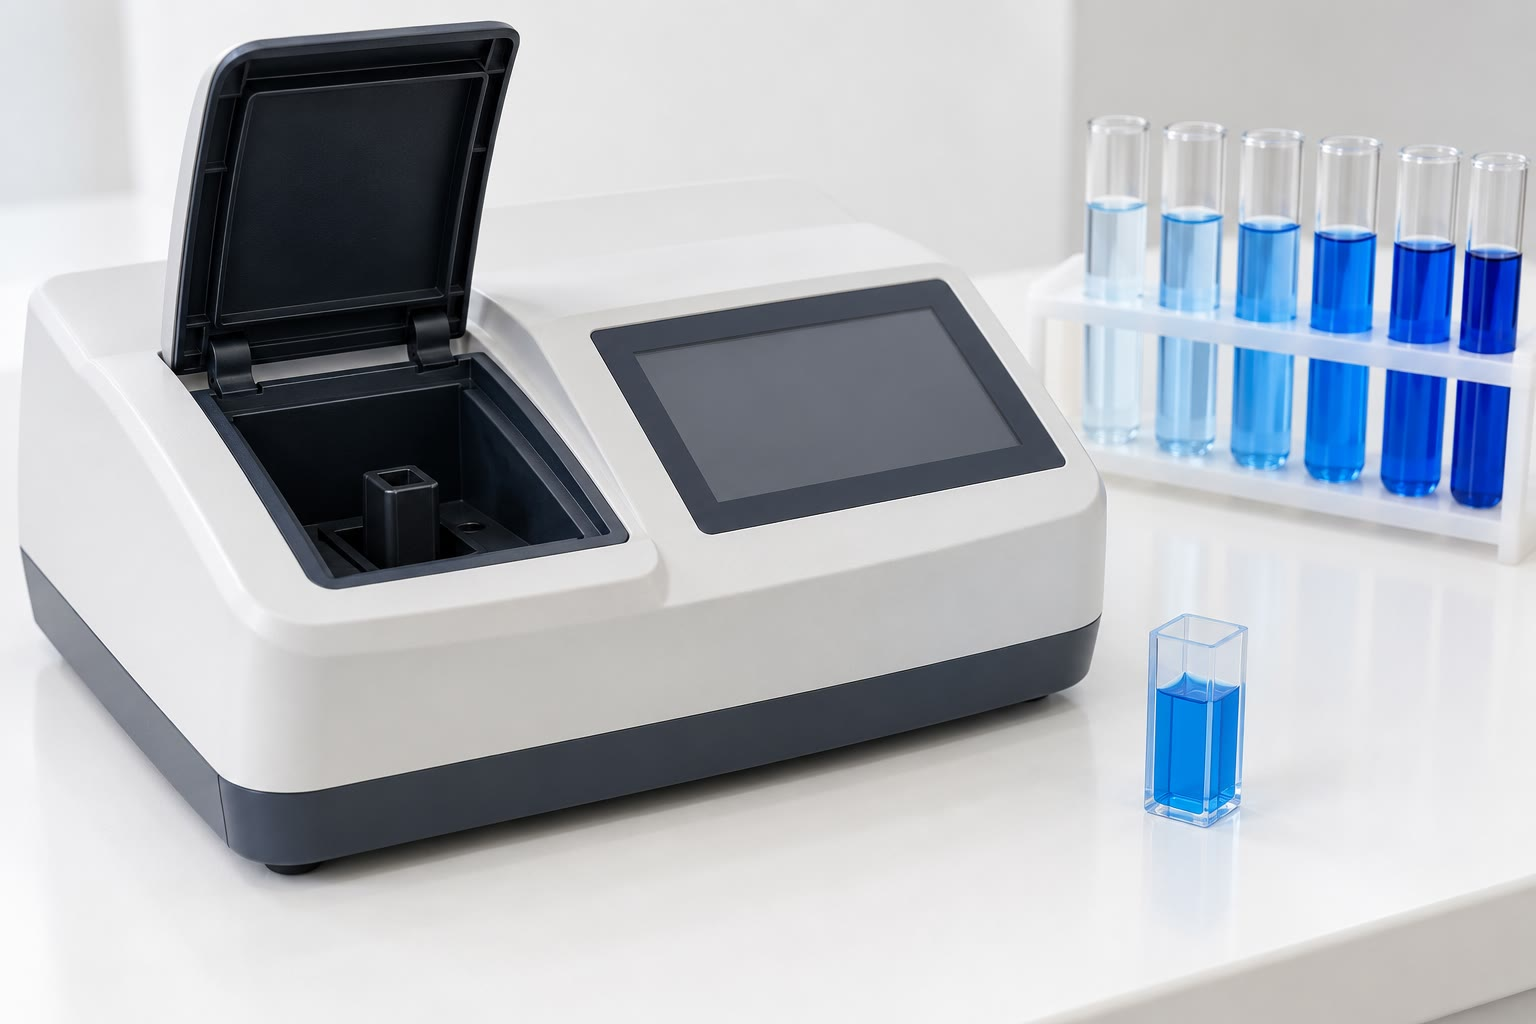
\includegraphics[width=0.5\linewidth]{images/book1/ai/g11-spectrophotometer.jpg}

{\small مطياف ضوئي وخلاياه المربعة.}
\end{omfigure}

\section{قانون بير--لامبرت}

\begin{definition}[معامل الامتصاص المولي]\label{def:g11:absorbance:epsilon}
\emph{معامل الامتصاص المولي}\index{معامل الامتصاص المولي}
$\varepsilon$ لنوع ذائب، عند طول موجة معيّن، يقيس شدة امتصاص \omterm{def:g10:the-mole:amount}{مول} واحد منه
للضوء؛ وهو يتوقف على النوع \omterm{def:g6:solutions-and-solubility:solute}{والمذيب} وطول الموجة، ويُعبَّر عنه
بوحدة \si{L/(mol.cm)}.
\end{definition}

\begin{proposition}[قانون بير--لامبرت]\label{prop:g11:absorbance:beer-lambert}
\omterm{def:g2:mixing-and-dissolving:dissolve}{لمحلول} مخفف فيه نوع ماصّ واحد تركيزه المولي $c$، في خلية سُمكها $\ell$،
تكون \omterm{def:g11:absorbance:absorbance}{الامتصاصية} عند طول موجة
معيّن
\[
  A = \varepsilon\, \ell\, c .
\]
\omterm{def:g11:absorbance:absorbance}{فالامتصاصية} تتناسب مع التركيز.
\end{proposition}

\begin{proof}
نقبله هنا؛ ويُشتق في أحد كتب المرحلة الجامعية.
\end{proof}


\begin{remark}[مع تركيز كتلي]\label{rem:g11:absorbance:mass}
% ledger: abs:E133, mw:E133
بما أن $c = C_m / M$، يمكن كتابة القانون أيضًا $A = a\, \ell\, C_m$،
حيث $a = \varepsilon / M$ بوحدة \si{L/(g.cm)}. والمواصفات الفنية للصبغات الغذائية
تعطي $a$: فللصبغة الزرقاء E133 عند \qty{629}{nm}، $a =
\qty{164}{L/(g.cm)}$، ومع كتلتها المولية \qty{792.9}{g/mol}،
$\varepsilon = 164 \times 792.9 = \qty{1.30e5}{L/(mol.cm)}$. \omterm{def:g2:mixing-and-dissolving:dissolve}{فمحلول} لا يحوي منها
إلا \qty{5.0}{mg/L}، في خلية من \qty{1}{cm}، يقرأ أصلًا
$A = 164 \times 1 \times 0.0050 = 0.82$.
\end{remark}

\begin{remark}[المحاليل المخففة فقط]\label{rem:g11:absorbance:dilute}
لا يصح التناسب إلا للمحاليل المخففة، أي عمليًا للامتصاصيات التي تقل عن نحو 1
إلى 1.5 في جهاز عادي. \omterm{def:g2:mixing-and-dissolving:dissolve}{والمحلول} الشديد التركيز يُخفَّف بمعامل معلوم قبل
قياسه.
\end{remark}

\section{قياس التركيز}

\begin{definition}[مستقيم المعايرة]\label{def:g11:absorbance:calibration-line}
\emph{مستقيم المعايرة}\index{مستقيم المعايرة} هو التمثيل البياني \omterm{def:g11:absorbance:absorbance}{لامتصاصية}
سلسلة من المحاليل المعيارية لنوع واحد، مقيسة عند طول الموجة نفسه وفي الخلية
نفسها، بدلالة تركيزها. وحين يصح قانون بير--لامبرت يكون خطًا مستقيمًا يمر
بالمبدأ.
\end{definition}

\begin{method}[قياس تركيز بمستقيم المعايرة]\label{met:g11:absorbance:calibration}
\begin{enumerate}
  \item سجّل طيف امتصاص النوع واختر طول الموجة
        $\lambda_{\max}$، حيث تكون \omterm{def:g11:absorbance:absorbance}{الامتصاصية} أكبر ما يمكن ويكون تغيّرها
        أقل ما يمكن مع خطأ صغير في طول الموجة.
  \item صفّر الجهاز بالشاهد.
  \item حضّر محاليل معيارية \omterm{def:g10:concentration-and-dilution:dilution}{بتخفيف} \omterm{def:g10:concentration-and-dilution:dilution}{محلول أم} وقِس
        امتصاصياتها.
  \item مثّل $A$ بدلالة التركيز وارسم المستقيم المار بالمبدأ الأقرب إلى
        النقاط.
  \item قِس المجهول، بعد تخفيفه إن لزم حتى تقع امتصاصيته بين امتصاصيات
        المحاليل المعيارية، واقرأ تركيزه على المستقيم (أو اقسم $A$ على
        الميل)؛ ثم اضربه في \omterm{def:g10:concentration-and-dilution:dilution}{معامل
        التخفيف}.
\end{enumerate}
\end{method}

\begin{omfigure}
\begin{tikzpicture}
\begin{axis}[width=0.72\linewidth, height=6cm, xmin=0, xmax=5.6,
    ymin=0, ymax=0.95, xlabel={\foreignlanguage{arabic}{تركيز \babelsublr{E133} \babelsublr{(\si{mg/L})}}},
    ylabel={\foreignlanguage{arabic}{الامتصاصية عند \qty{629}{nm}}}, axis lines*=left, ymajorgrids,
    xmajorgrids, grid style={gray!20}, tick label style={font=\small},
    label style={font=\small}]
  % ledger: abs:E133 (points synthetic: exact values + fixed offsets)
  \addplot[only marks, mark=*, mark size=2.2pt, omDef] table[x=C, y=A]
    {figdata/out/grade-11-absorbance-b.dat};
  \addplot[thick, omProp, domain=0:5.5] {0.164*x};
  \addplot[dashed, black!60] coordinates {(0,0.590) (3.6,0.590) (3.6,0)};
  \node[font=\small, anchor=south west] at (axis cs:0.1,0.6) {\foreignlanguage{arabic}{المجهول: $A = 0.590$}};
  \node[font=\small, anchor=west] at (axis cs:3.65,0.22) {\qty{3.6}{mg/L}};
\end{axis}
\end{tikzpicture}

{\small مستقيم معايرة الصبغة الزرقاء: خمسة محاليل معيارية (النقاط) والمستقيم المار
بالمبدأ، وميله \qty{0.164}{L/mg}. فالمجهول الذي يقرأ $A = 0.590$ تركيزه
$0.590 / 0.164 =
\qty{3.6}{mg/L}$.}
\end{omfigure}

\begin{example}[المحاليل المعيارية الخمسة]\label{ex:g11:absorbance:standards}
يُخفَّف \omterm{def:g10:concentration-and-dilution:dilution}{محلول أم} من الصبغة الزرقاء تركيزه \qty{100}{mg/L} لتحضير
\qty{100.0}{mL} من كل \omterm{def:g10:concentration-and-dilution:standard}{محلول معياري}: فلمحلول \qty{2.0}{mg/L} يكون \omterm{def:g10:concentration-and-dilution:dilution}{معامل
التخفيف} 50، فيُكمَّل \qty{2.0}{mL} من \omterm{def:g10:concentration-and-dilution:dilution}{المحلول الأم} حتى \qty{100.0}{mL}.
والمحاليل المعيارية الخمسة، من 1 إلى \qty{5}{mg/L}، تقرأ 0.168 و0.325 و0.494
و0.652 و0.823: أي في حدود بضعة أجزاء من ألف من $0.164 \times C$، مستقيم
الشكل.
\end{example}

\section{تمارين}

\begin{exercise}[$\star$]\label{exo:g11:absorbance:1}
\omterm{def:g2:mixing-and-dissolving:dissolve}{محلول} يمتص أساسًا الضوء البرتقالي. بأي لون يبدو؟ \omterm{def:g2:mixing-and-dissolving:dissolve}{ومحلول} يمتص أساسًا الضوء
البنفسجي؟
\end{exercise}

\begin{exercise}[$\star$]\label{exo:g11:absorbance:2}
مستعينًا بدائرة الألوان، أعطِ اللون الذي يمتصه أساسًا \omterm{def:g2:mixing-and-dissolving:dissolve}{محلول} أخضر، ومجال أطوال
الموجات التي يغطيها ذلك اللون.
\end{exercise}

\begin{exercise}[$\star$]\label{exo:g11:absorbance:3}
اقرأ على طيفي الامتصاص طول الموجة $\lambda_{\max}$ لكل صبغة
وامتصاصيتها عنده.
\end{exercise}

\begin{exercise}[$\star$]\label{exo:g11:absorbance:4}
\omterm{def:g2:mixing-and-dissolving:dissolve}{محلول} صبغة تركيزه \qty{2.0}{mg/L} يقرأ $A = 0.30$. فماذا يقرأ \omterm{def:g2:mixing-and-dissolving:dissolve}{محلول} للصبغة
نفسها تركيزه \qty{6.0}{mg/L} في الخلية نفسها وعند طول الموجة
نفسه؟ وعند \qty{1.0}{mg/L}؟
\end{exercise}

\begin{exercise}[$\star$]\label{exo:g11:absorbance:5}
ما شاهد المطياف الضوئي، ولماذا يُصفَّر الجهاز
به؟
\end{exercise}

\begin{exercise}[$\star\star$]\label{exo:g11:absorbance:6}
مستعينًا بمستقيم معايرة الصبغة الزرقاء، جد تركيز \omterm{def:g2:mixing-and-dissolving:dissolve}{محلول} يقرأ
$A = 0.41$.
\end{exercise}

\begin{exercise}[$\star\star$]\label{exo:g11:absorbance:7}
لقياس الصبغة الزرقاء، لماذا يُضبط المطياف الضوئي على
\qty{629}{nm} لا على \qty{550}{nm}؟ أعطِ سببين.
\end{exercise}

\begin{exercise}[$\star\star$]\label{exo:g11:absorbance:8}
مشروب غير مخفف يقرأ $A = 2.4$ عند \qty{629}{nm}، وهي قيمة أعلى من أن يوثق بها.
فيُخفَّف خمس مرات فيقرأ عندئذ $A = 0.48$. جد تركيز الصبغة الزرقاء في
المشروب.
\end{exercise}

\begin{exercise}[$\star\star$]\label{exo:g11:absorbance:9}
% ledger: mw:E102, abs:E102
\omterm{def:g2:mixing-and-dissolving:dissolve}{محلول} من التارترازين تركيزه \qty{15.0}{mg/L} يقرأ $A = 0.795$ عند
\qty{427}{nm} في خلية سُمكها \qty{1.00}{cm}. احسب معامل امتصاصه الكتلي $a$ بوحدة
\si{L/(g.cm)}، ثم معامل امتصاصه المولي (\omterm{def:g10:the-mole:molar-mass}{الكتلة المولية}
\qty{534.4}{g/mol}).
\end{exercise}

\begin{exercise}[$\star\star$]\label{exo:g11:absorbance:10}
انظر إلى طيفي الصبغتين. فوق أي طول موجة لا تكاد الصبغة الصفراء تمتص شيئًا؟
ولماذا يمكن قياس الصبغة الزرقاء عند \qty{629}{nm} حتى في مشروب أخضر يحوي
الصبغة الصفراء أيضًا؟
\end{exercise}

\begin{exercise}[$\star\star$]\label{exo:g11:absorbance:11}
يُقاس \omterm{def:g2:mixing-and-dissolving:dissolve}{المحلول} نفسه في خلية سُمكها \qty{2.0}{cm} بدلًا من
\qty{1.0}{cm}. كيف تتغير امتصاصيته؟ ولماذا؟
\end{exercise}

\begin{exercise}[$\star\star\star$]\label{exo:g11:absorbance:12}
محاليل معيارية من الصبغة الزرقاء تراكيزها 5 و10 و20 و\qty{40}{mg/L} تقرأ 0.82
و1.62 و2.30 و2.70. احسب $A / C$ لكل منها. ماذا تلاحظ؟ وأي المحاليل المعيارية
يمكن استعمالها \omterm{def:g11:absorbance:calibration-line}{لمستقيم المعايرة}، وماذا يجب أن يُفعل بمجهول يقرأ
$2.5$؟
\end{exercise}

\begin{exercise}[$\star\star\star$]\label{exo:g11:absorbance:13}
مشروب أخضر يحوي الصبغة الزرقاء والصبغة الصفراء. في خلية سُمكها
\qty{1.00}{cm} يقرأ $A = 0.574$ عند \qty{629}{nm} و$A = 0.53$
عند \qty{427}{nm}. وعند \qty{427}{nm} لا تكاد الصبغة الزرقاء تمتص شيئًا،
وعند \qty{629}{nm} لا تمتص الصبغة الصفراء شيئًا. جد التركيزين الكتليين
للصبغتين (استعمل $a = \qty{164}{L/(g.cm)}$
و$a = \qty{53.0}{L/(g.cm)}$).
\end{exercise}

\begin{exercise}[$\star\star\star$]\label{exo:g11:absorbance:14}
تنسى تلميذة الشاهد فتصفّر الجهاز بخلية فارغة. فتصير كل قراءة أعلى بمقدار
\num{0.040}. ويقرأ المجهول $0.368$، فتقسم على الميل $0.164$ \omterm{def:g11:absorbance:calibration-line}{لمستقيم
المعايرة} الحقيقي. ما التركيز الذي تجده؟ وما التركيز الحقيقي؟ وبأي نسبة مئوية
تخطئ؟
\end{exercise}

\begin{exercise}[$\star\star\star$]\label{exo:g11:absorbance:15}
% ledger: adi:E102
الكمية اليومية المقبولة من التارترازين \qty{10}{mg} لكل كيلوغرام من كتلة الجسم.
ومشروب يحوي منه \qty{20}{mg/L}. ما حجم المشروب الذي يبلغ ببالغ كتلته
\qty{60}{kg} هذه الكمية في يوم واحد؟ وهل هذا خطر واقعي؟
\end{exercise}

\section{مسألة: زرقة مشروب رياضي}


\begin{problem}[{مسألة نهاية الأسبوع --- كم قارورة من مشروب رياضي أزرق
يجب أن يشرب طفل ليبلغ الحد اليومي الآمن من
صبغته؟}]
\label{pb:g11:absorbance:1}
% ledger: lmax:E133, abs:E133, mw:E133, adi:E133
يتحقق مختبر أغذية من الصبغة الزرقاء E133 في مشروب رياضي يُباع في قوارير
من \qty{500}{mL}. وتعطي المواصفات الفنية للصبغة كتلتها المولية،
\qty{792.9}{g/mol}، وكميتها اليومية المقبولة: \qty{6}{mg} لكل
كيلوغرام من كتلة الجسم في اليوم، وهو مقدار يمكن تناوله كل يوم مدى الحياة
دون خطر يُذكر.

\medskip
\noindent\textbf{الجزء الأول --- اللون والطيف.}
\begin{enumerate}
  \item يبدو المشروب أزرق. مستعينًا بدائرة الألوان، أي لون من الضوء يمتصه
        أكثر من غيره؟
  \item اقرأ طول الموجة $\lambda_{\max}$ للصبغة على طيفها.
  \item لماذا تكاد \omterm{def:g11:absorbance:absorbance}{امتصاصية} الصبغة تنعدم عند \qty{450}{nm}؟
        وهل يتفق ذلك مع لونها؟
  \item عند أي طول موجة يجب أن تُجرى القياسات؟
\end{enumerate}

\medskip
\noindent\textbf{الجزء الثاني --- \omterm{def:g11:absorbance:calibration-line}{مستقيم المعايرة}.}
\begin{enumerate}[resume]
  \item تُذاب \qty{50.0}{mg} من الصبغة النقية لتحضير \qty{500.0}{mL}
        من \omterm{def:g10:concentration-and-dilution:dilution}{المحلول الأم}. احسب تركيزه الكتلي بوحدة \si{mg/L}.
  \item تُحضَّر محاليل معيارية تراكيزها 1.0 و2.0 و3.0 و4.0 و\qty{5.0}{mg/L}،
        \qty{100.0}{mL} من كل منها. ما حجم \omterm{def:g10:concentration-and-dilution:dilution}{المحلول الأم} اللازم \omterm{def:g10:concentration-and-dilution:standard}{للمحلول
        المعياري} \qty{3.0}{mg/L}؟ وبأي أدوات زجاجية؟
  \item تقرأ المحاليل المعيارية 0.168 و0.325 و0.494 و0.652 و0.823. احسب
        $A / C$ لكل منها، وبيّن أن النقاط تقع قريبًا من مستقيم يمر
        بالمبدأ ميله نحو \qty{0.164}{L/mg}.
  \item لماذا يجب أن يمر المستقيم بالمبدأ؟
  \item استنتج معامل الامتصاص الكتلي $a$ للصبغة بوحدة \si{L/(g.cm)} (خلية
        سُمكها \qty{1.00}{cm})، ثم معامل امتصاصها المولي.
\end{enumerate}

\medskip
\noindent\textbf{الجزء الثالث --- المشروب.}
\begin{enumerate}[resume]
  \item يُكمَّل \qty{25.0}{mL} من المشروب حتى \qty{50.0}{mL} بالماء.
        ما \omterm{def:g10:concentration-and-dilution:dilution}{معامل التخفيف}؟
  \item يقرأ المشروب المخفف $A = 0.590$. جد تركيزه من
        الصبغة.
  \item استنتج تركيز الصبغة في المشروب نفسه.
  \item ماذا كان سيقرأ المشروب غير المخفف؟ ولماذا خُفّف؟
  \item احسب كتلة الصبغة في قارورة واحدة.
  \item احسب \omterm{def:g10:the-mole:amount}{كمية مادة} الصبغة، \omterm{def:g10:the-mole:amount}{بالمول}، في قارورة واحدة.
\end{enumerate}

\medskip
\noindent\textbf{الجزء الرابع --- الكمية اليومية المقبولة.}
\begin{enumerate}[resume]
  \item ما كتلة الصبغة التي يجوز لطفل كتلته \qty{30}{kg} أن يتناولها في
        اليوم؟
  \item كم قارورة يجب أن يشرب الطفل في يوم واحد ليبلغها؟
  \item ما حجم المشروب الذي يمثله ذلك؟ علّق.
  \item السؤال نفسه لبالغ كتلته \qty{70}{kg}.
  \item اذكر الجواب النهائي: كم قارورة من \qty{500}{mL} يجب أن يشرب طفل
        كتلته \qty{30}{kg} في يوم ليبلغ الكمية اليومية المقبولة من
        الصبغة؟
\end{enumerate}
\end{problem}
